\documentclass[11pt, a4paper]{article}
\usepackage{pdfpages}
\usepackage{parallel}
\usepackage[T2A]{fontenc}
\usepackage{ucs}
\usepackage[utf8x]{inputenc}
\usepackage[polish,english,russian]{babel}
\usepackage{hyperref}
\usepackage{rotating}
\usepackage[inner=2cm,top=1.8cm,outer=2cm,bottom=2.3cm,nohead]{geometry}
\usepackage{listings}
\usepackage{graphicx}
\usepackage{wrapfig}
\usepackage{longtable}
\usepackage{indentfirst}
\usepackage{array}
\usepackage{tikzsymbols}
\usepackage{soul}
\usepackage[ruled,vlined]{algorithm2e}
%\counterwithout{figure}{section} 

\usepackage{url}
\makeatletter
\g@addto@macro{\UrlBreaks}{\UrlOrds}
\makeatother

\newcolumntype{P}[1]{>{\raggedright\arraybackslash}p{#1}}
\frenchspacing
\usepackage{fixltx2e} %text sub- and superscripts
\usepackage{icomma} % коскі ў матэматычным рэжыме
\PreloadUnicodePage{4}

\newcommand{\longpage}{\enlargethispage{\baselineskip}}
\newcommand{\shortpage}{\enlargethispage{-\baselineskip}}

\def\switchlang#1{\expandafter\csname switchlang#1\endcsname}
\def\switchlangbe{
\let\saverefname=\refname%
\def\refname{Літаратура}%
\def\figurename{Іл.}%
}
\def\switchlangen{
\let\saverefname=\refname%
\def\refname{References}%
\def\figurename{Fig.}%
}
\def\switchlangru{
\let\saverefname=\refname%
\let\savefigurename=\figurename%
\def\refname{Литература}%
\def\figurename{Рис.}%
}

\hyphenation{admi-ni-stra-tive}
\hyphenation{ex-pe-ri-ence}
\hyphenation{fle-xi-bi-li-ty}
\hyphenation{Py-thon}
\hyphenation{ma-the-ma-ti-cal}
\hyphenation{re-ported}
\hyphenation{imp-le-menta-tions}
\hyphenation{pro-vides}
\hyphenation{en-gi-neering}
\hyphenation{com-pa-ti-bi-li-ty}
\hyphenation{im-pos-sible}
\hyphenation{desk-top}
\hyphenation{elec-tro-nic}
\hyphenation{com-pa-ny}
\hyphenation{de-ve-lop-ment}
\hyphenation{de-ve-loping}
\hyphenation{de-ve-lop}
\hyphenation{da-ta-ba-se}
\hyphenation{plat-forms}
\hyphenation{or-ga-ni-za-tion}
\hyphenation{pro-gramming}
\hyphenation{in-stru-ments}
\hyphenation{Li-nux}
\hyphenation{sour-ce}
\hyphenation{en-vi-ron-ment}
\hyphenation{Te-le-pathy}
\hyphenation{Li-nux-ov-ka}
\hyphenation{Open-BSD}
\hyphenation{Free-BSD}
\hyphenation{men-ti-on-ed}
\hyphenation{app-li-ca-tion}

\def\progref!#1!{\texttt{#1}}
\renewcommand{\arraystretch}{2} %Іначай формулы ў матрыцы зліпаюцца з лініямі
\usepackage{array}

\def\interview #1 (#2), #3, #4, #5\par{

\section[#1, #3, #4]{#1 -- #3, #4}
\def\qname{LVEE}
\def\aname{#1}
\def\q ##1\par{{\noindent \bf \qname: ##1 }\par}
\def\a{{\noindent \bf \aname: } \def\qname{L}\def\aname{#2}}
}

\def\interview* #1 (#2), #3, #4, #5\par{

\section*{#1\\{\small\rm #3, #4. #5}}
\ifx\ParallelWhichBox\undefined%
    \addcontentsline{toc}{section}{#1, #3, #4}%
\else%
\ifnum\ParallelWhichBox=0%
    \addcontentsline{toc}{section}{#1, #3, #4}%
\fi\fi%

\def\qname{LVEE}
\def\aname{#1}
\def\q ##1\par{{\noindent \bf \qname: ##1 }\par}
\def\a{{\noindent \bf \aname: } \def\qname{L}\def\aname{#2}}
}

\newcommand{\interviewfooter}[1]{
\vskip 1em
\noindent \textit{#1}
}

\switchlang{en}
\begin{document}

\title{1995 "--- Logitech TrackMan Marble trackball}
\date{}
\maketitle
\selectlanguage{english}
The Trackman Marble trackball (figure \ref{fig:trackman}), released to the market by Logitech in 1995, was the first trackball to use an all-optical motion detection principle, without the use of an optomechanical encoder \cite{logitech25}.

\begin{figure}[h]
    \centering
    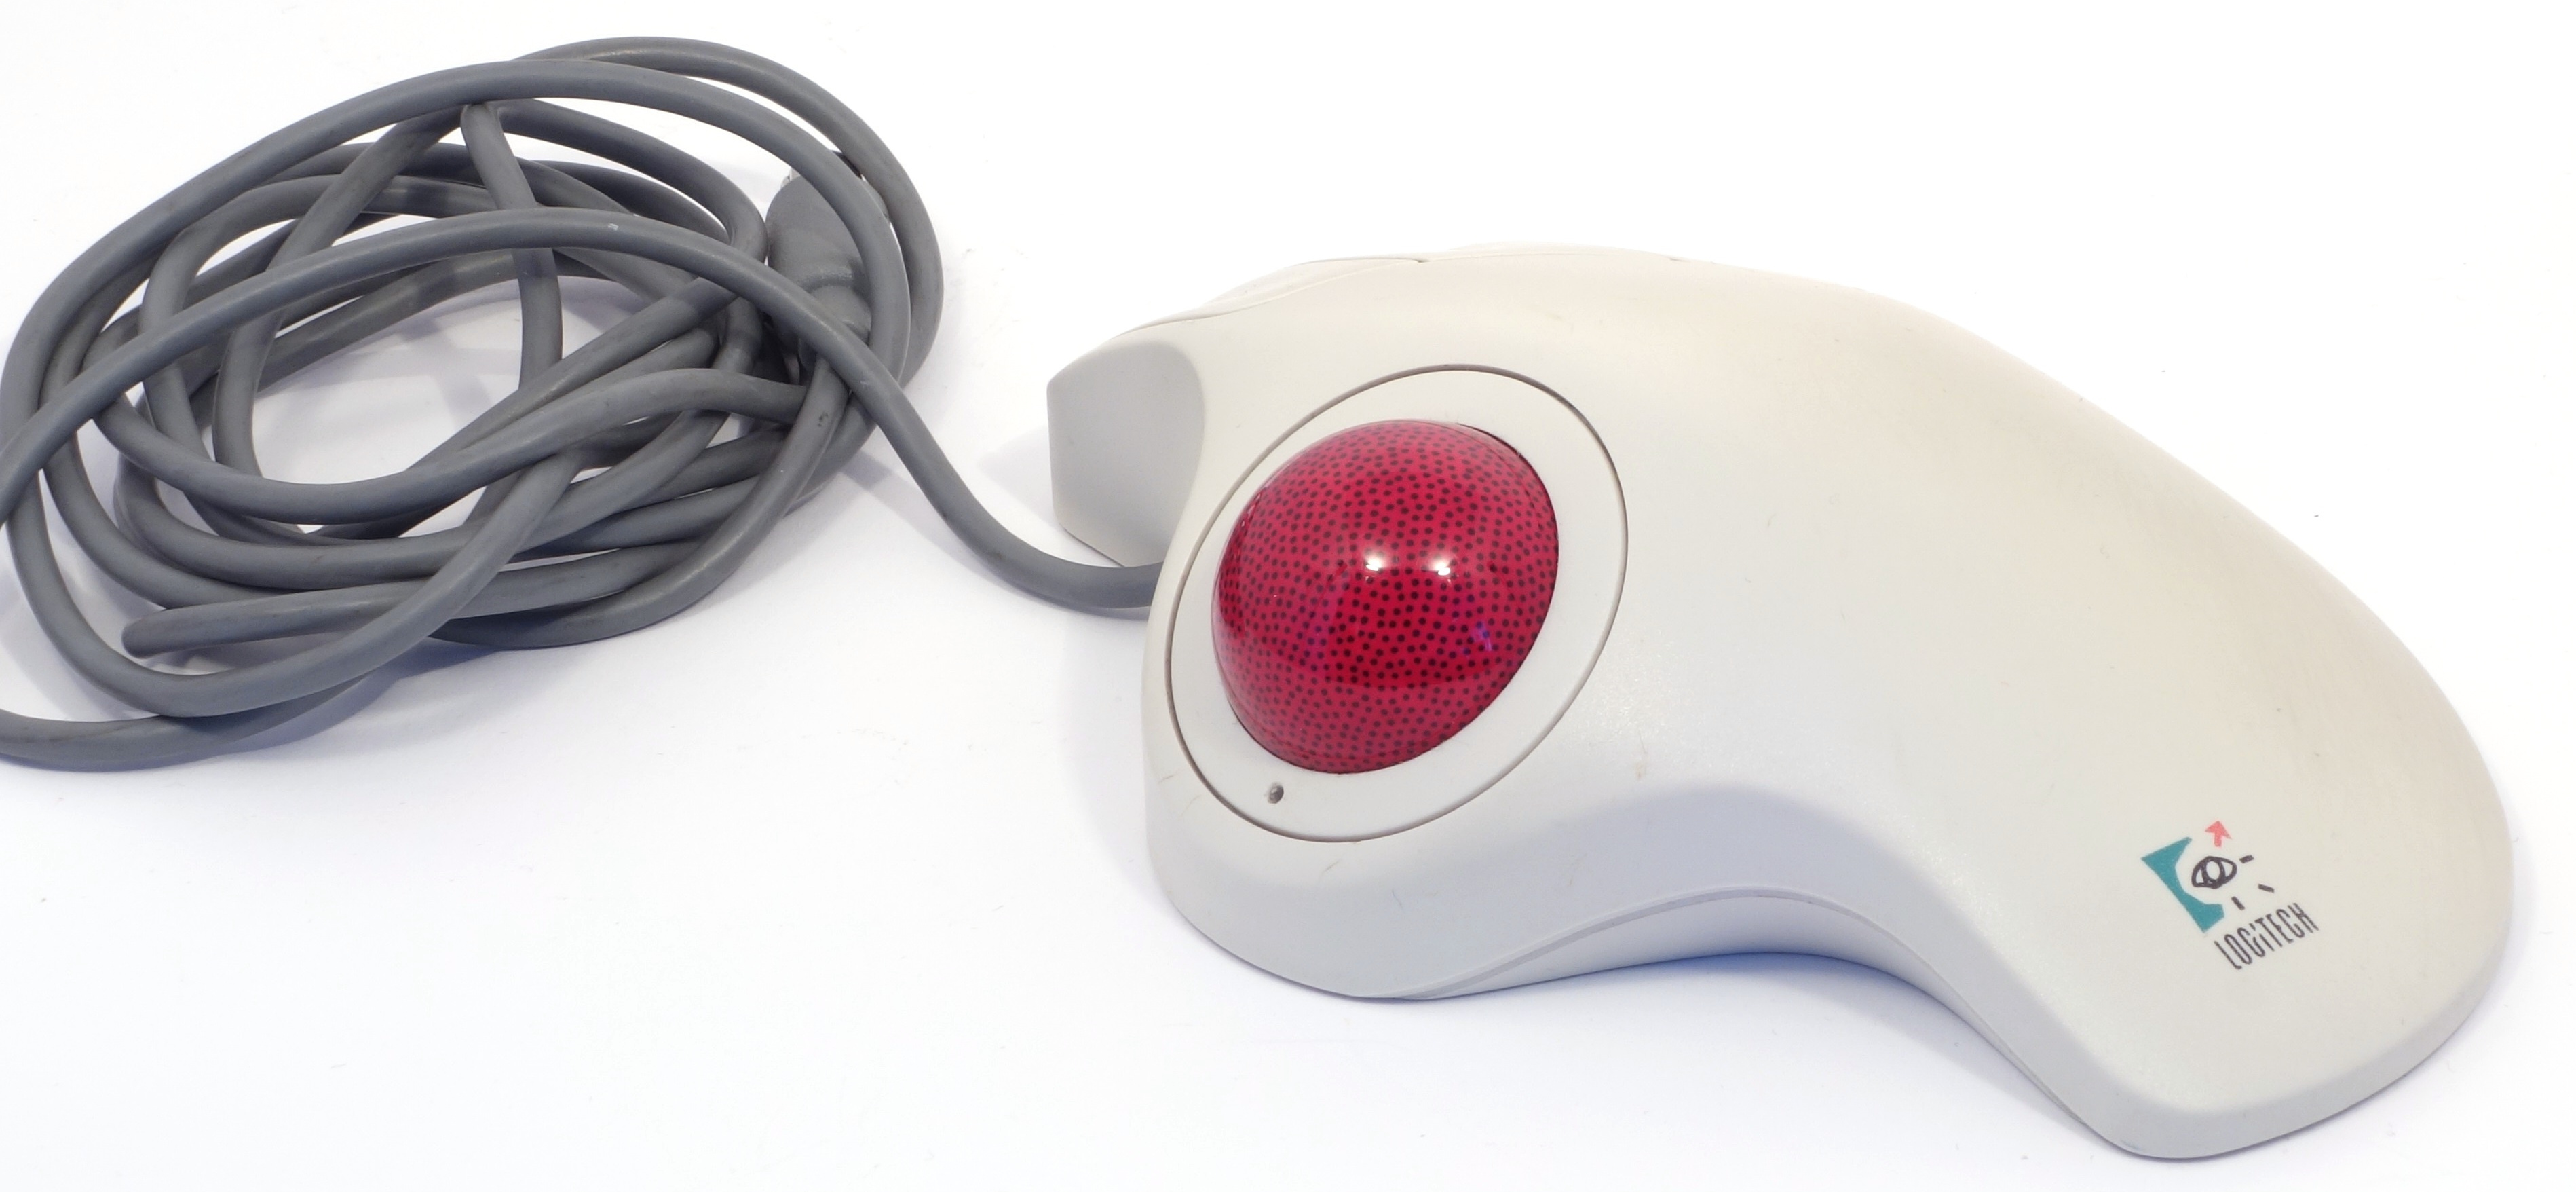
\includegraphics[scale=0.45]{1995_logitech_trackman/pic_60.jpg}
    \caption{Logitech TrackMan Marble trackball}
    \label{fig:trackman}
\end{figure}

This trackball has three keys, which are the standard three mouse buttons, and a ball positioned to be rotated by the right thumb (figure \ref{fig:trackmanTopAndBottom}). A regular pattern of dark dots on the surface of the ball is needed for an optical sensor. There is no scroll wheel on this model, but the driver allowed using the rotation of the ball with the middle button pressed to scroll (single presses of this button performs the usual middle button function). It should be noted that there was also a modification of this trackball with a scroll wheel in the cutout of the third button. The trackball is connected to the computer via the PS/2 interface.

\begin{figure}[h]
    \centering
    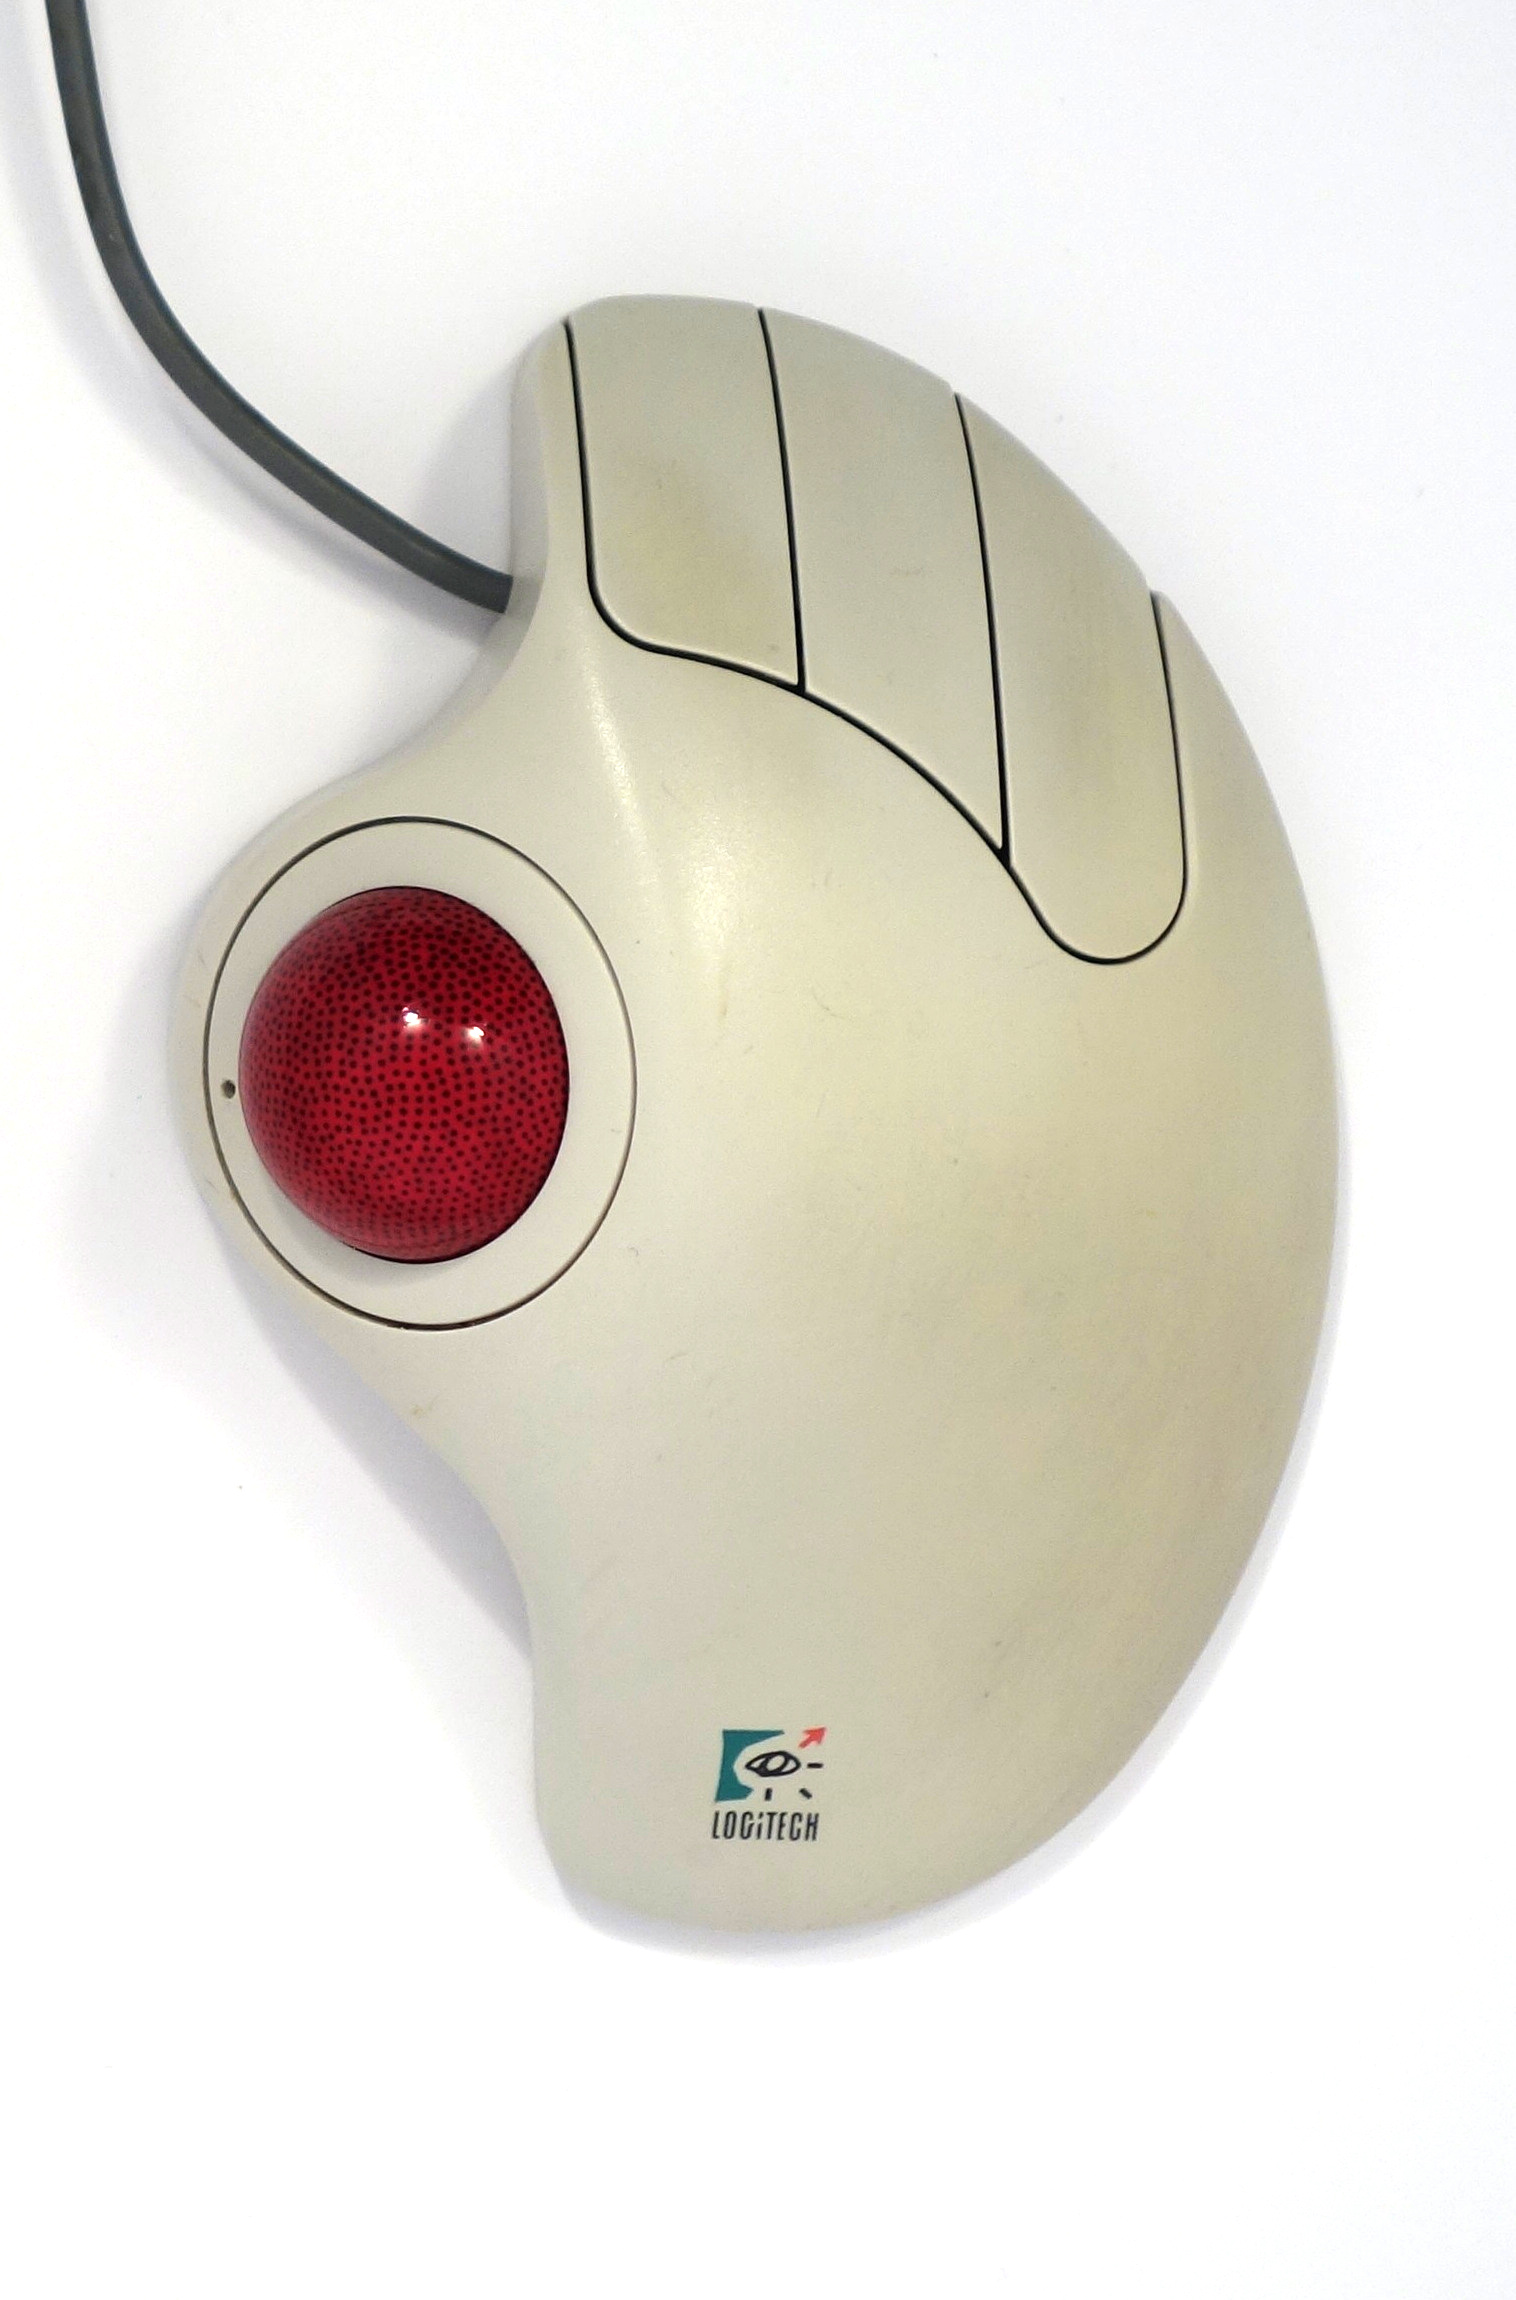
\includegraphics[scale=0.4]{1995_logitech_trackman/top_60.jpg}
    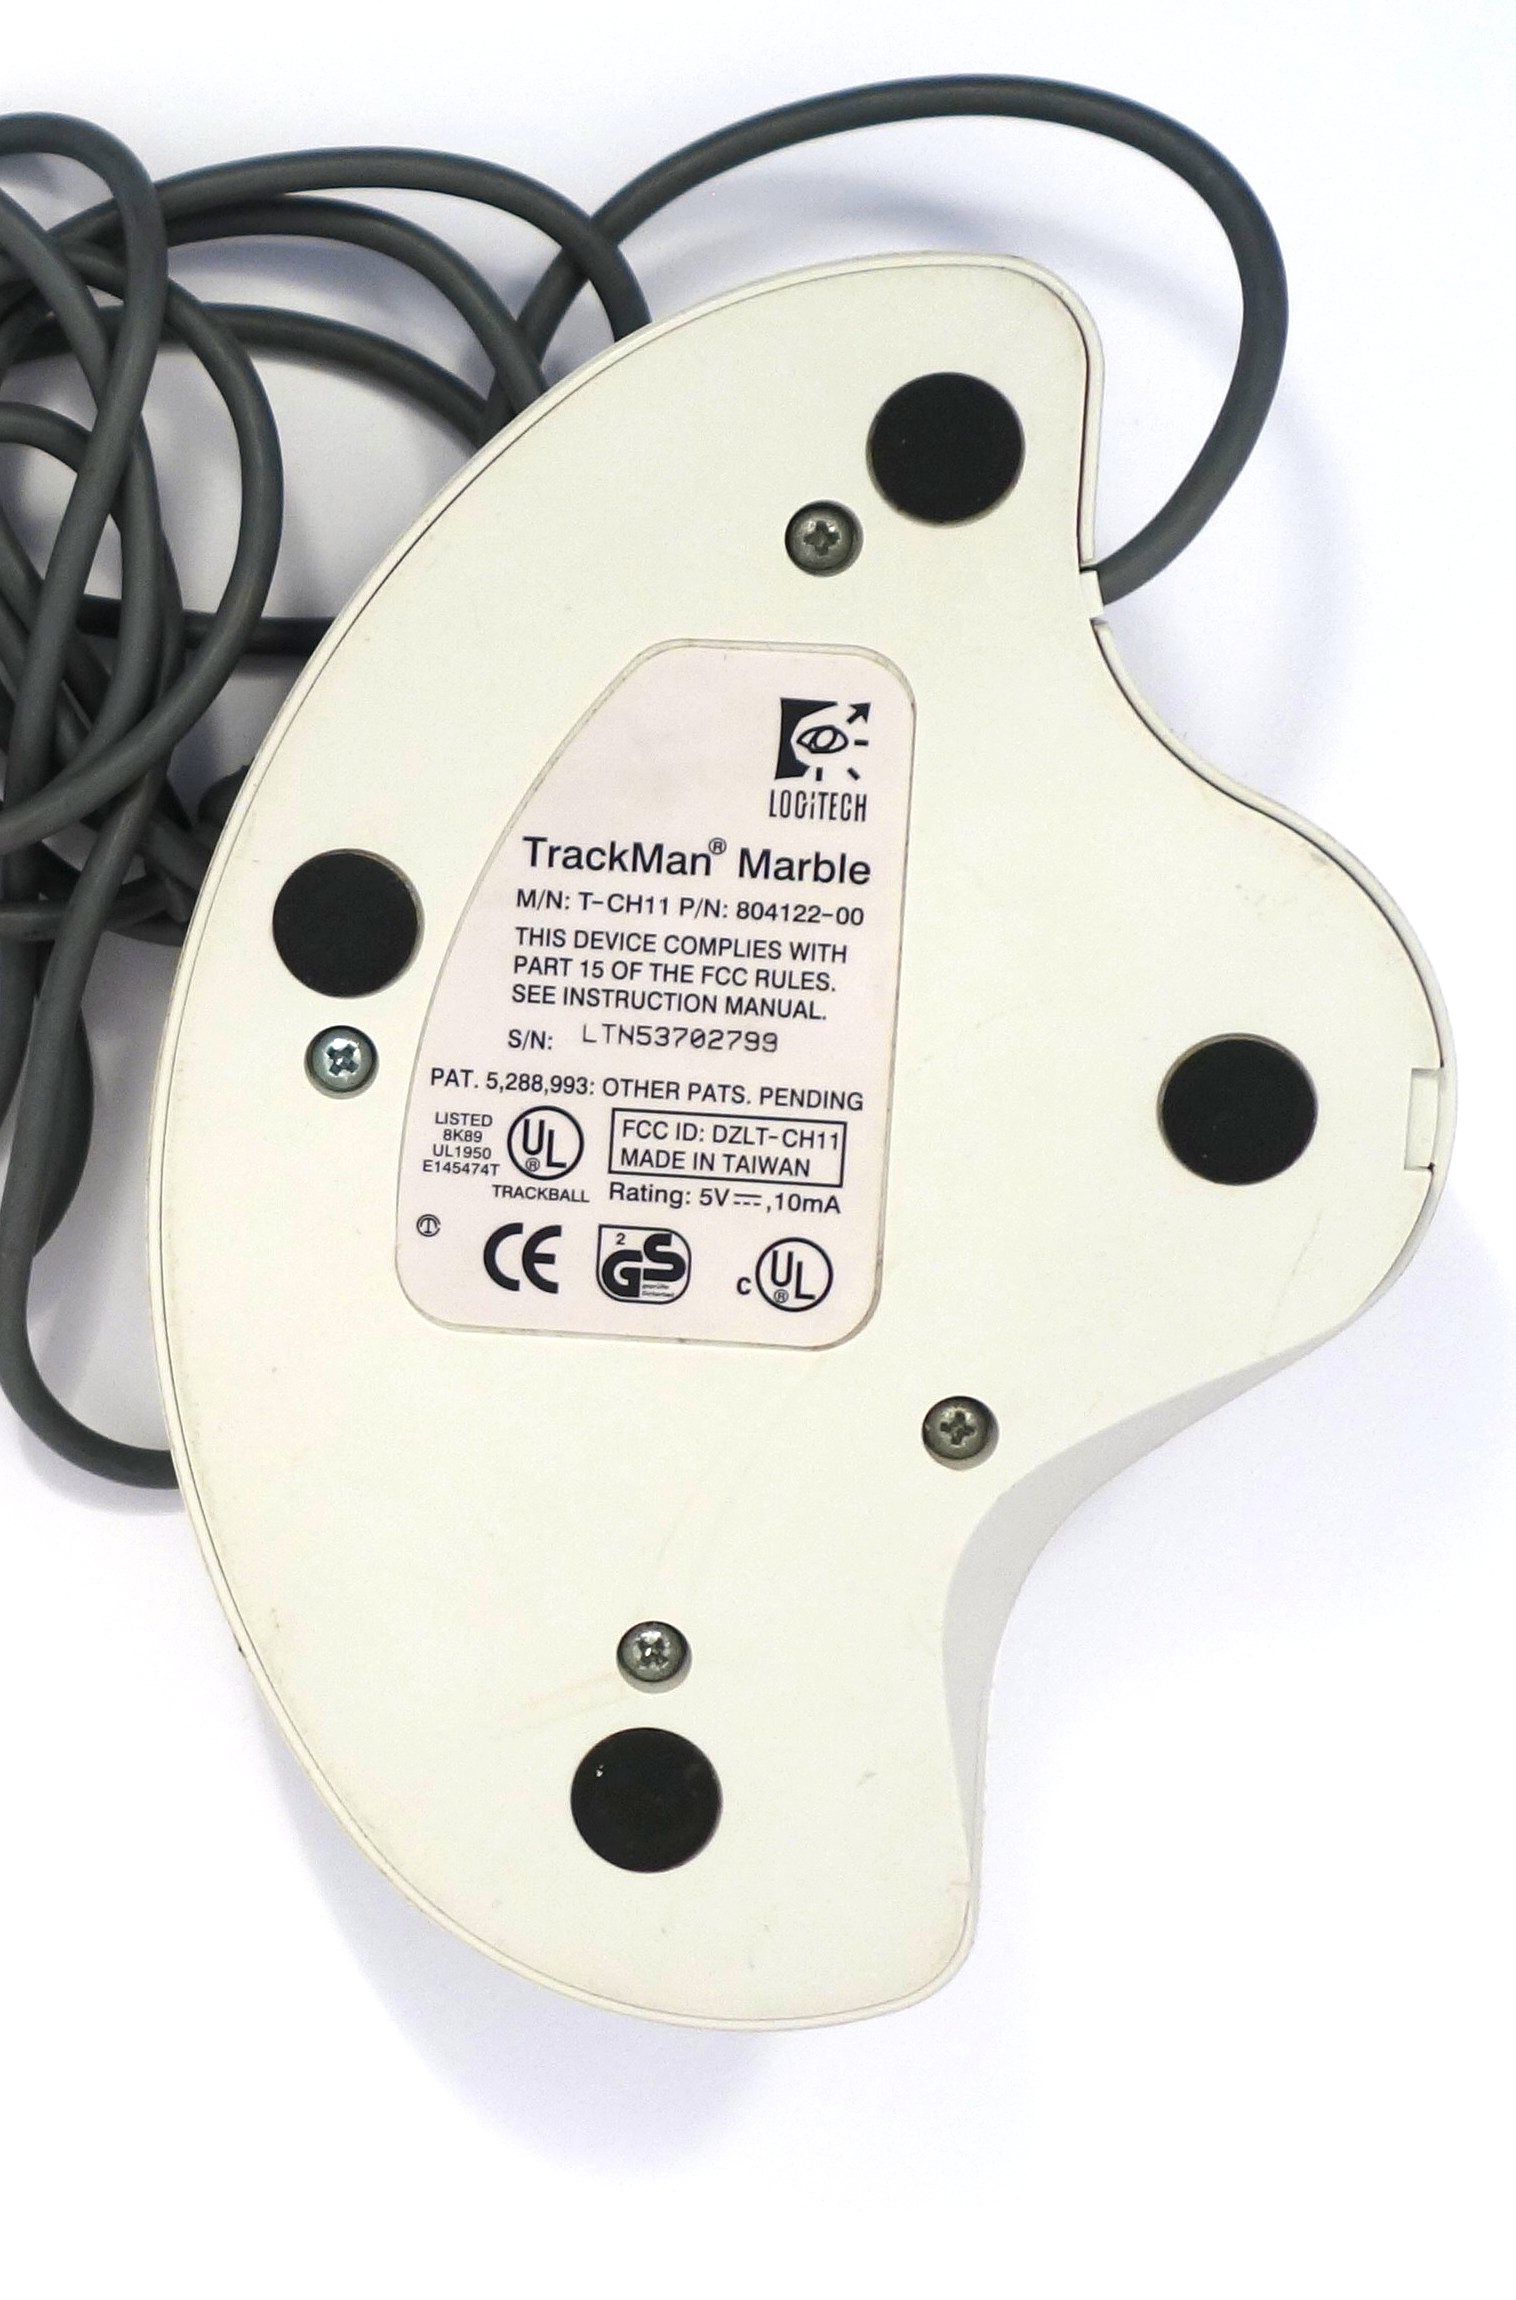
\includegraphics[scale=0.4]{1995_logitech_trackman/bottom_60.jpg}
    \caption{Logitech TrackMan, top and bottom views}
    \label{fig:trackmanTopAndBottom}
\end{figure}

\begin{figure}[h]
    \centering
    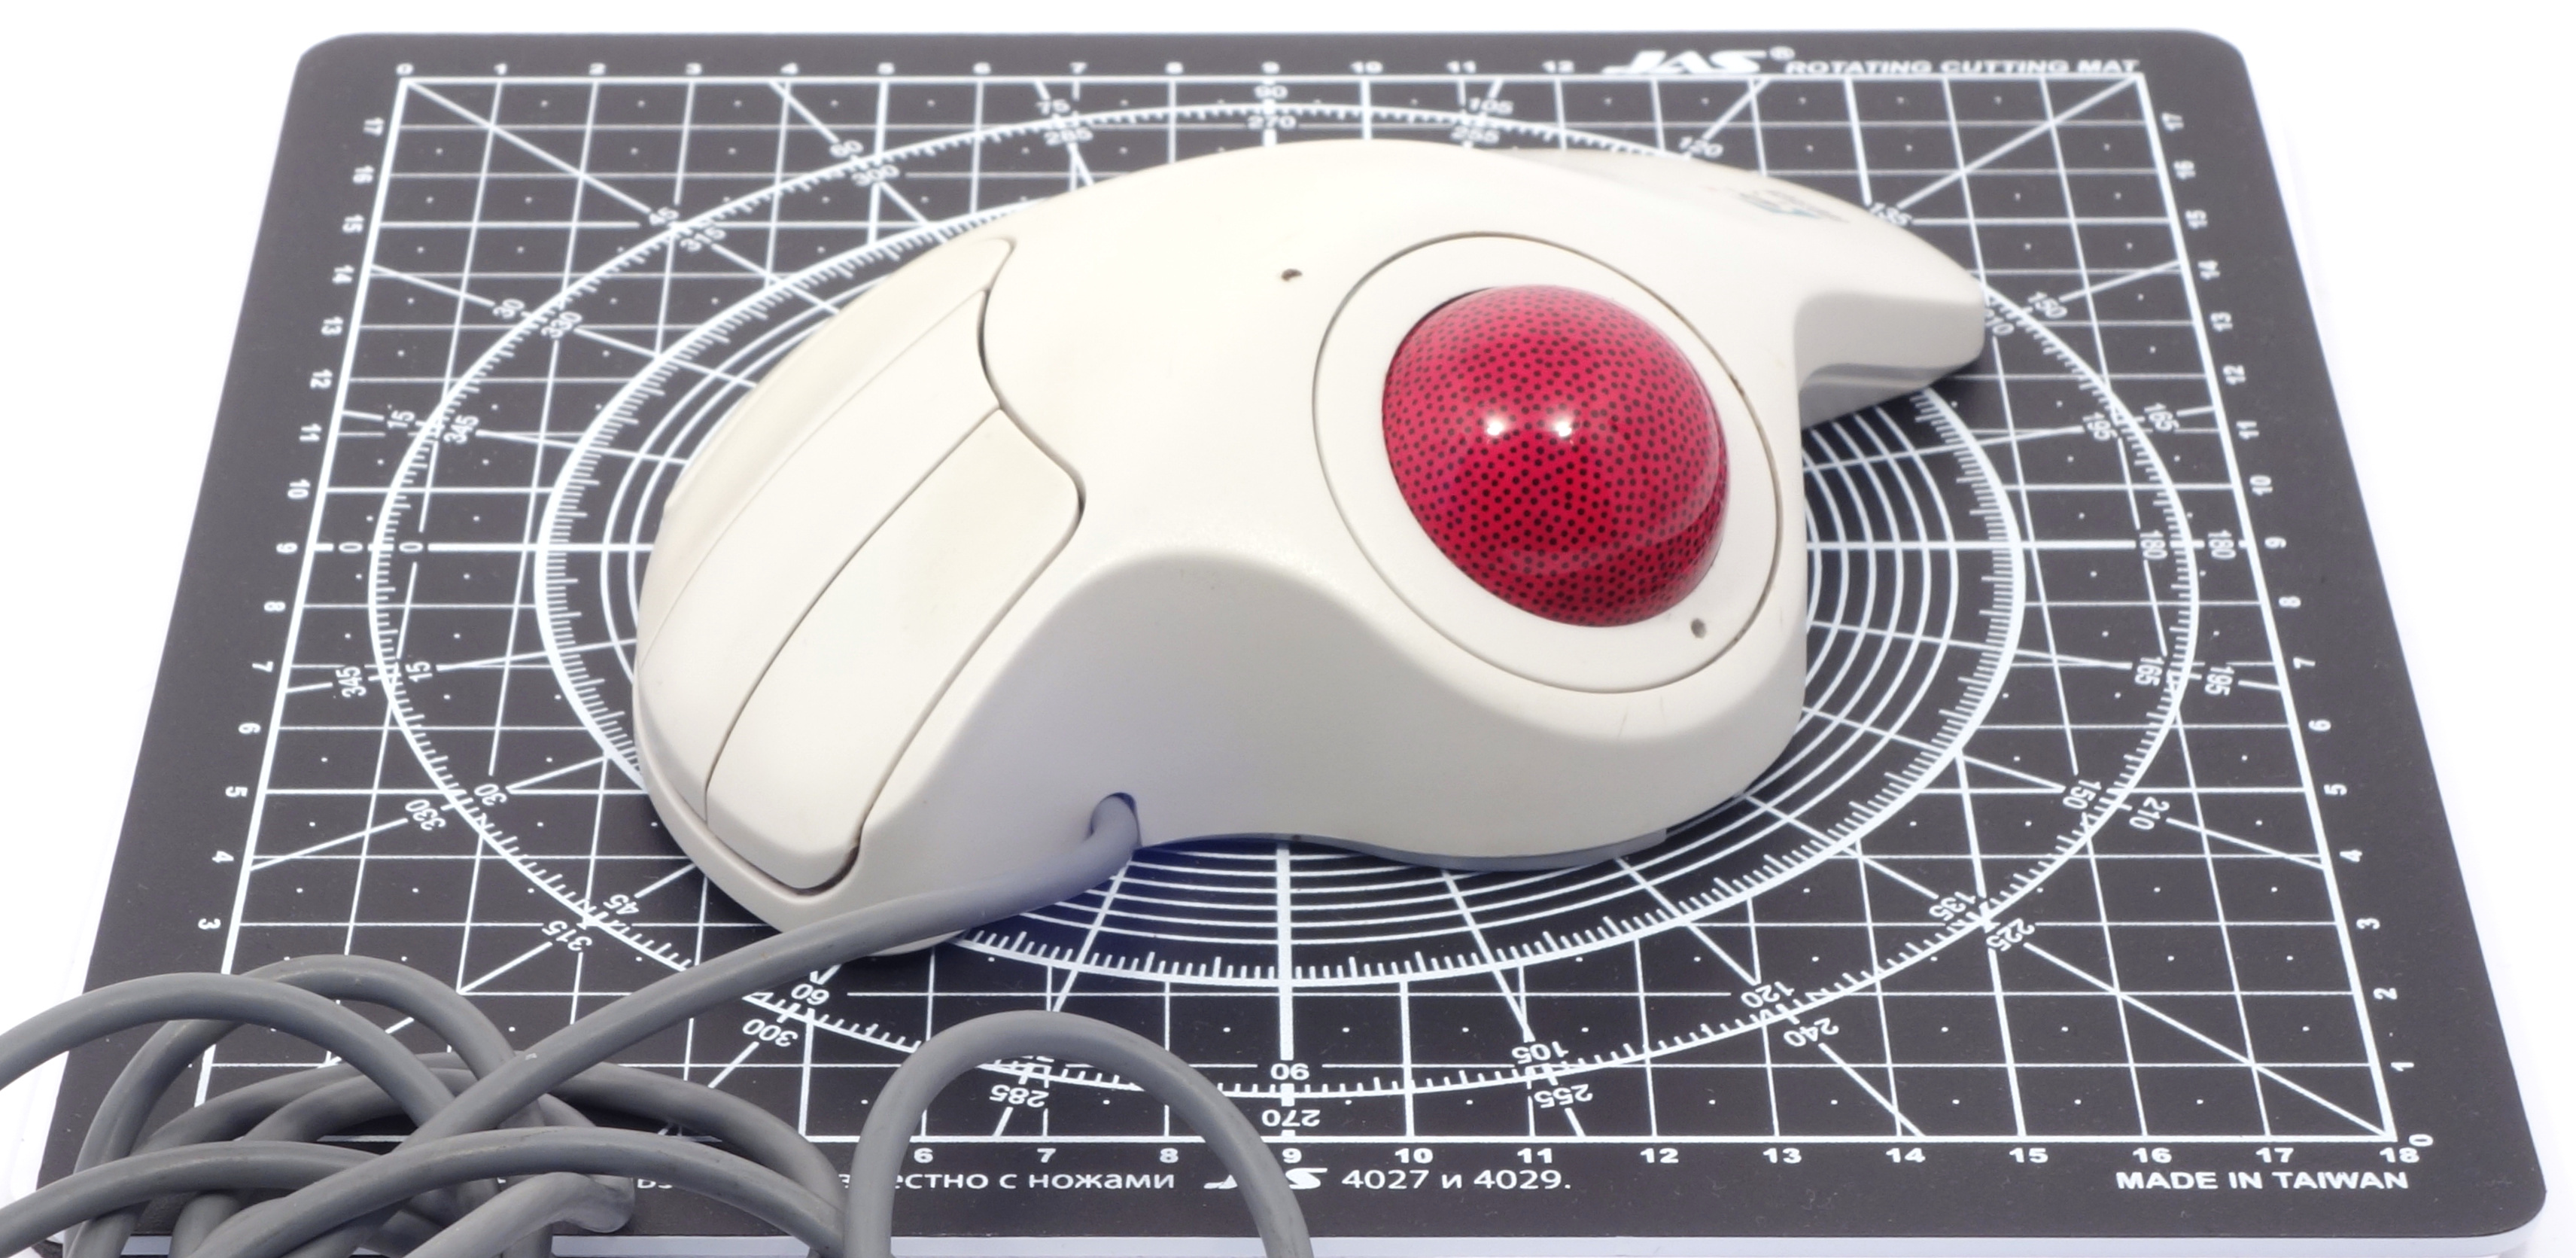
\includegraphics[scale=0.4]{1995_logitech_trackman/size_30.jpg}
    \caption{Logitech TrackMan on a graduated pad with a grid step of 1~cm}
    \label{fig:trackmanSize}
\end{figure}

The trackball is medium in size (figure \ref{fig:trackmanSize}). Most of the trackball's body is slanted to the right, which puts the user's wrist in a more natural position. While the ball is scrolled by the thumb, the rest of the fingers work in the same way as with a conventional mouse, which makes the design more attractive for a user who has often used the mouse before or alternately uses the mouse and trackball (figure \ref{fig:trackmanHand}). However, this arrangement also has disadvantages: the thumb is not the most agile and accurate finger, which theoretically can affect the speed and accuracy of positioning. In addition, due to this form, the device is completely unsuitable for left-handers.

\begin{figure}[h]
    \centering
    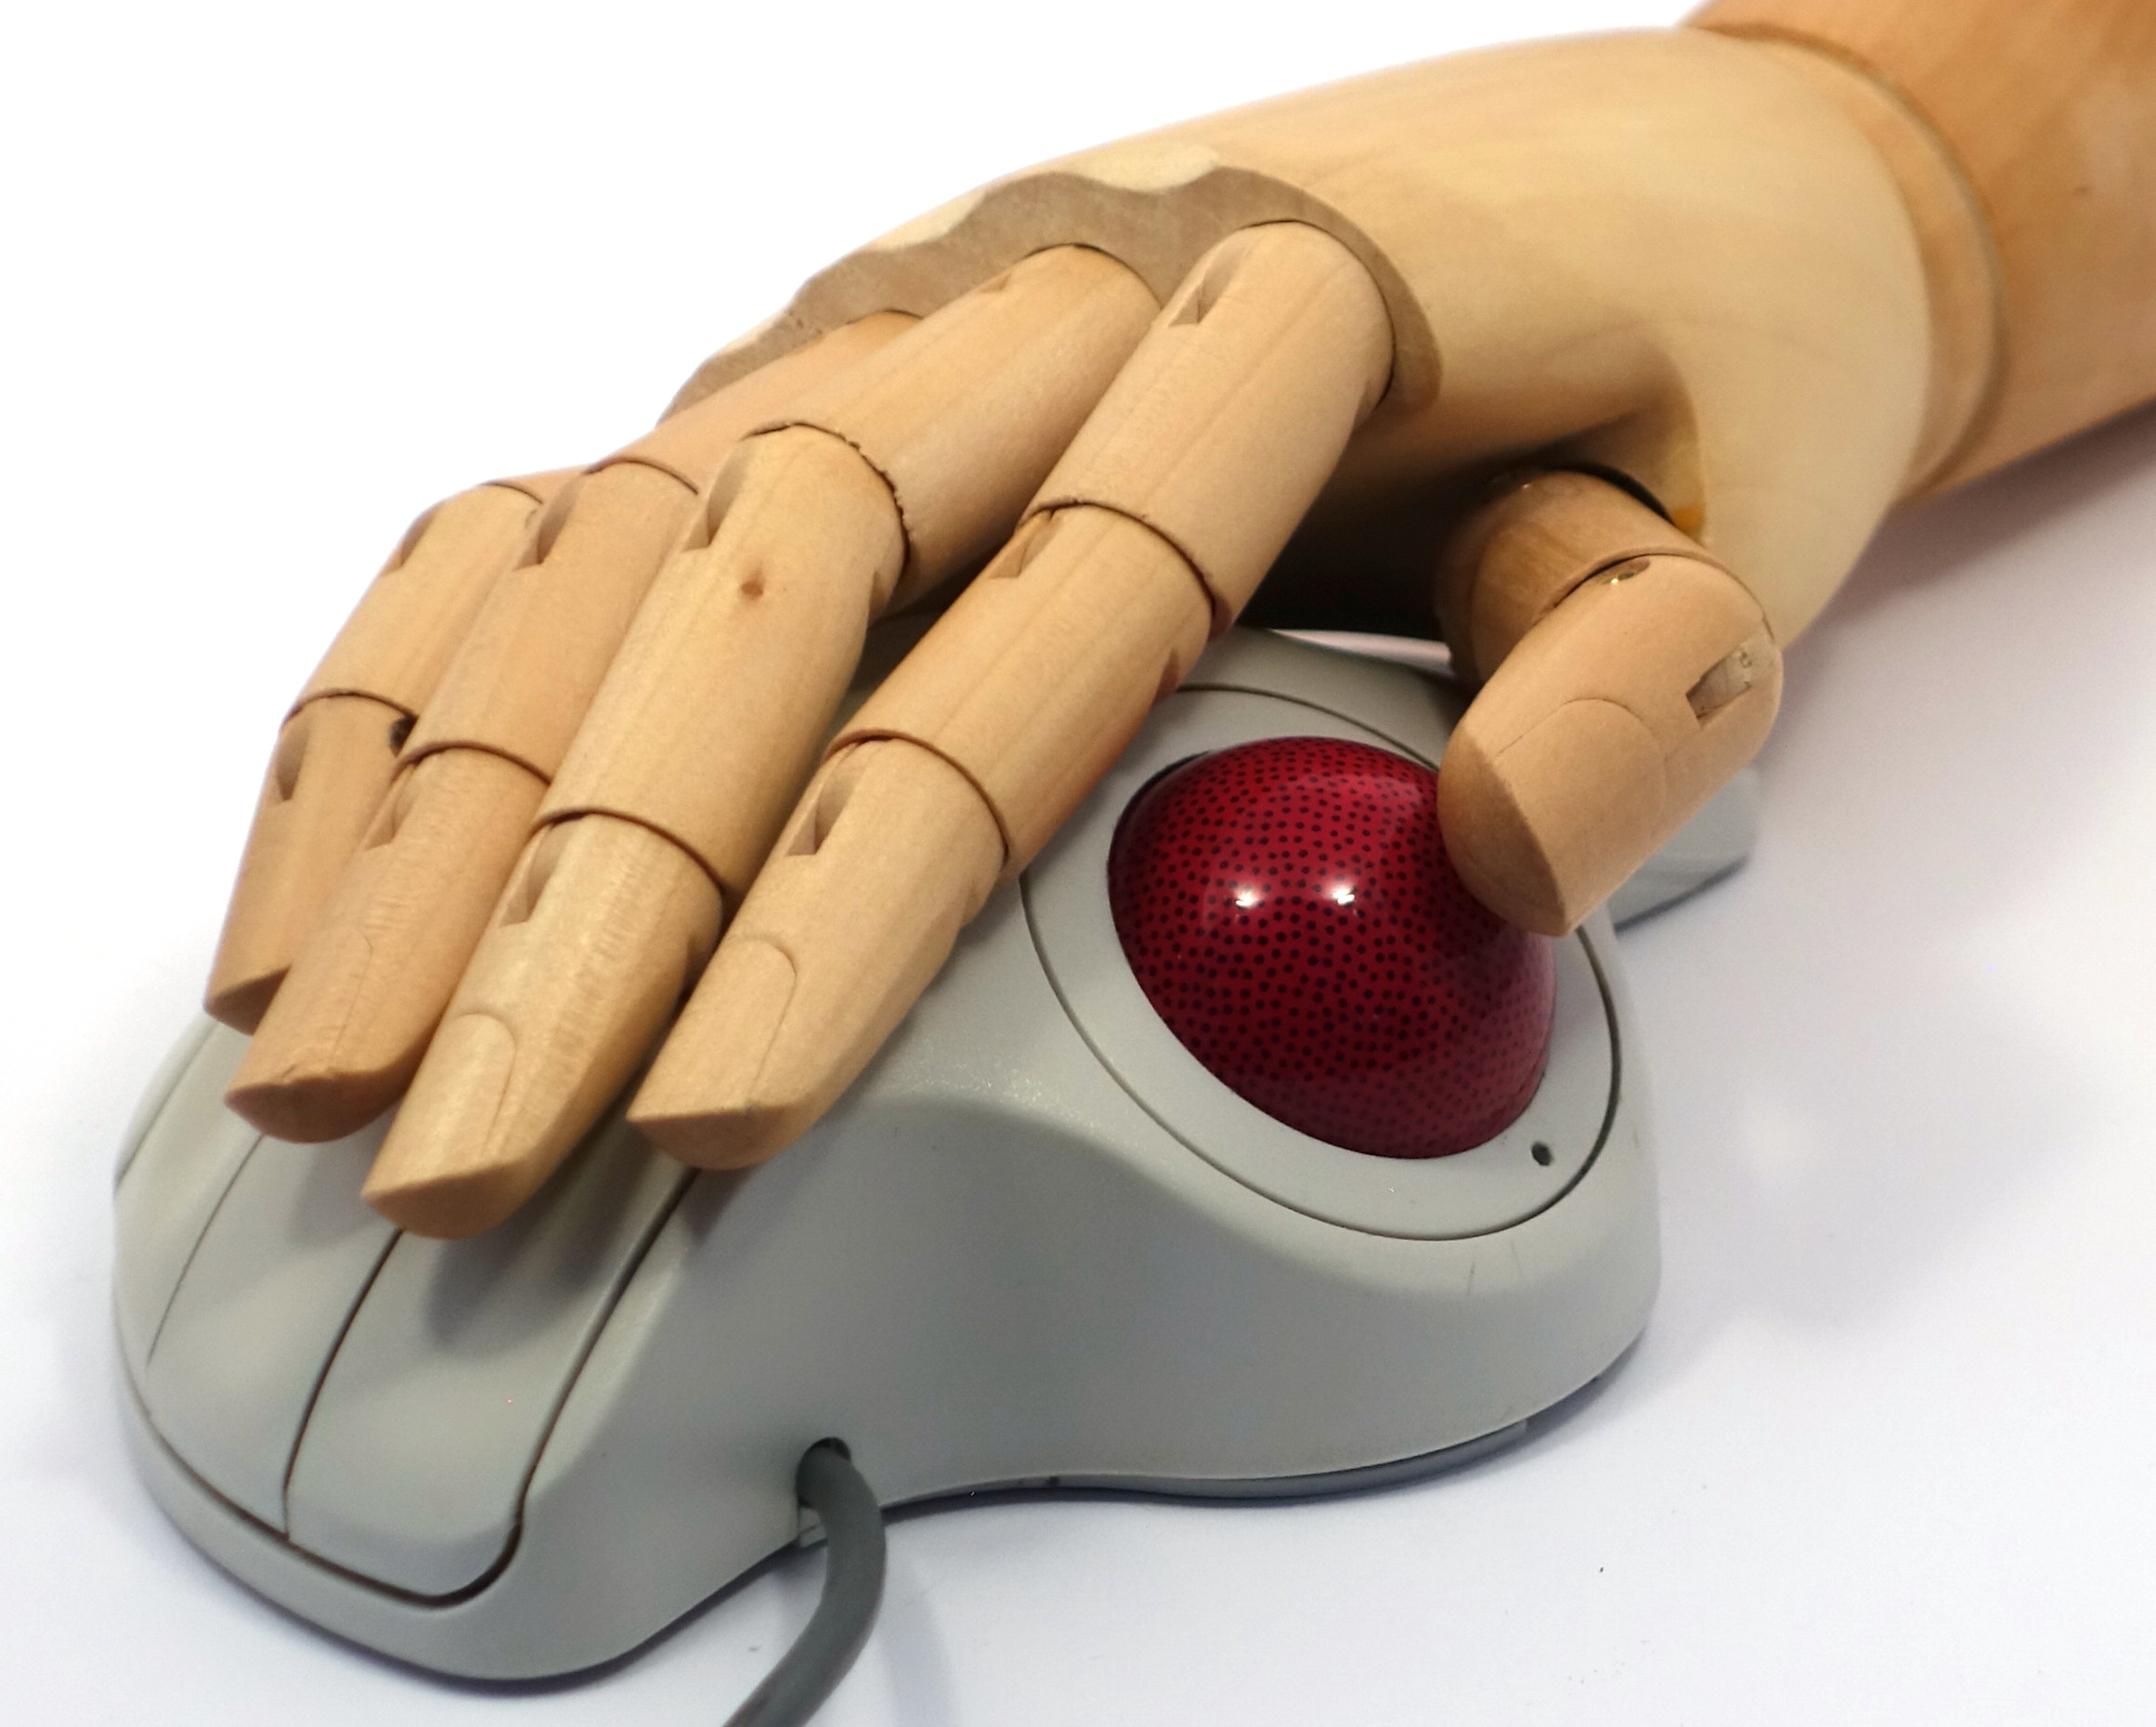
\includegraphics[scale=0.6]{1995_logitech_trackman/hand_30.jpg}
    \caption{Logitech TrackMan trackball with a human hand model}
    \label{fig:trackmanHand}
\end{figure}

Trackball internals are shown on figure \ref{fig:trackmanInside}. The reason that Logitech has changed the color of the ball is clearly visible. In fact, instead of the traditional opto-mechanical scheme, this trackball turned out to be the first one built according to the optical mouse, when the changes in brightness are detected using a special mouse pad with a grid drawn on it (in this case, a pattern on a rotating ball plays the role of a pad). According to developers, movement recognition is implemented by a system based on an artificial neural network \cite{marbleAdv}.

\begin{figure}[h]
    \centering
    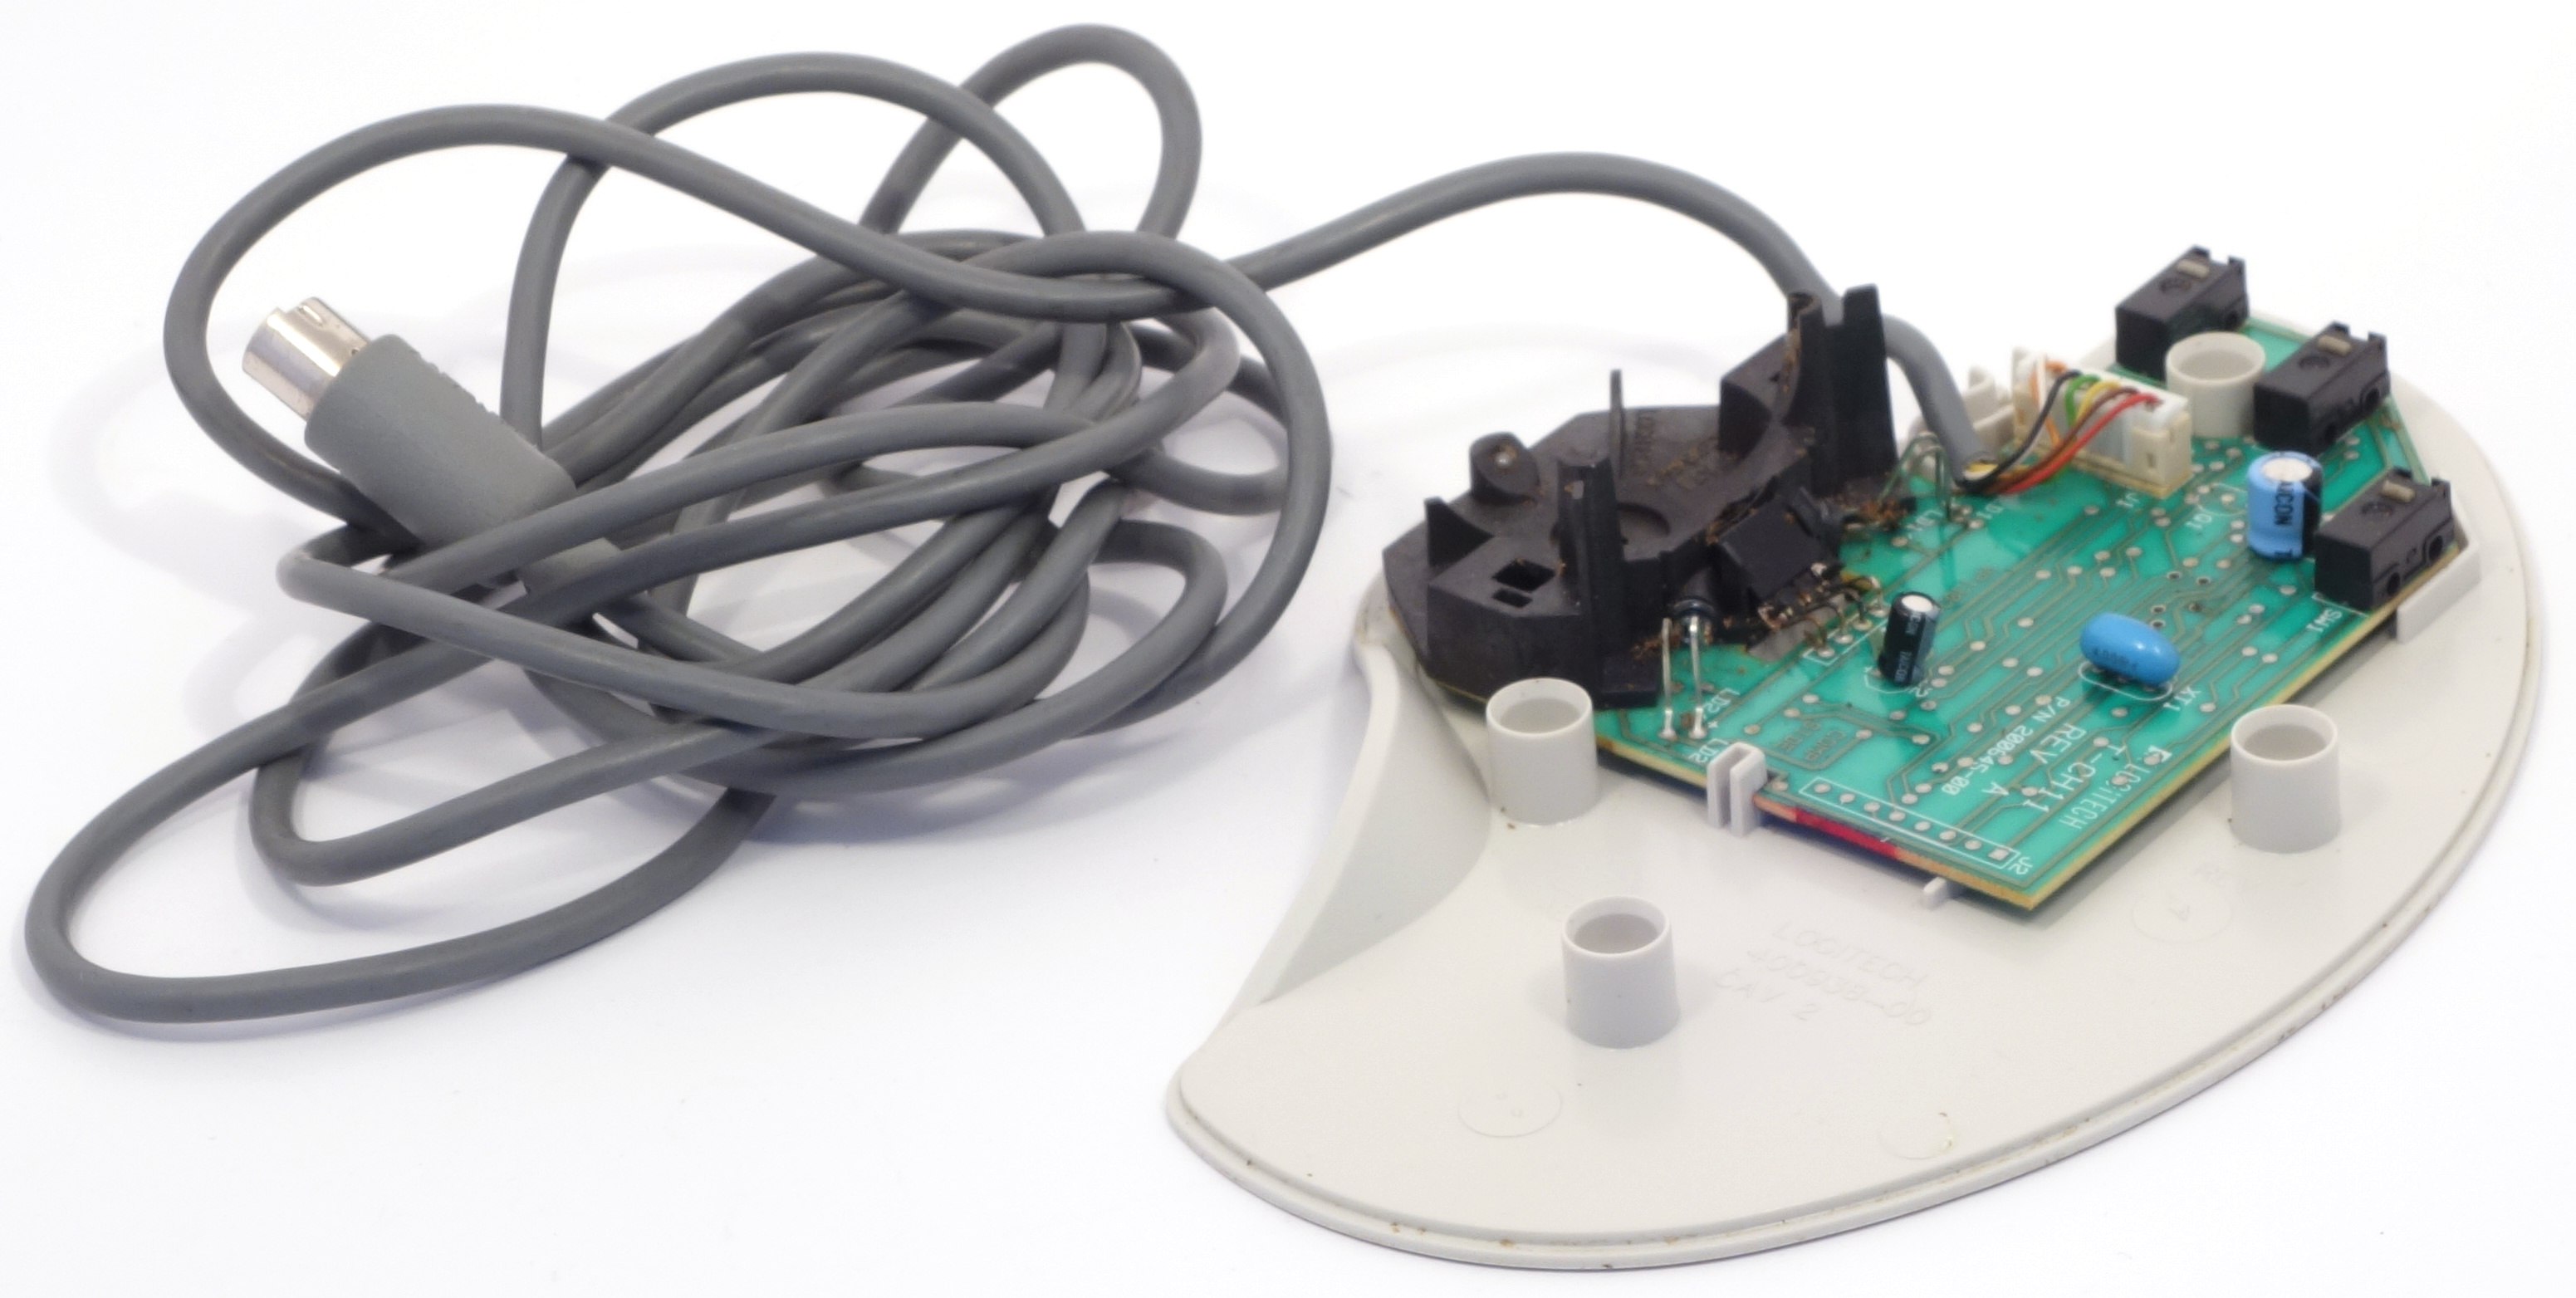
\includegraphics[scale=0.6]{1995_logitech_trackman/inside_30.jpg}
    \caption{Logitech TrackMan trackball disassembled}
    \label{fig:trackmanInside}
\end{figure}

 The FCC ID code (Figure \ref{fig:trackmanTopAndBottom}) reveals that this mouse was manufactured by the Logitech company in 1995.

%\begin{figure}[h]
%    \centering
%    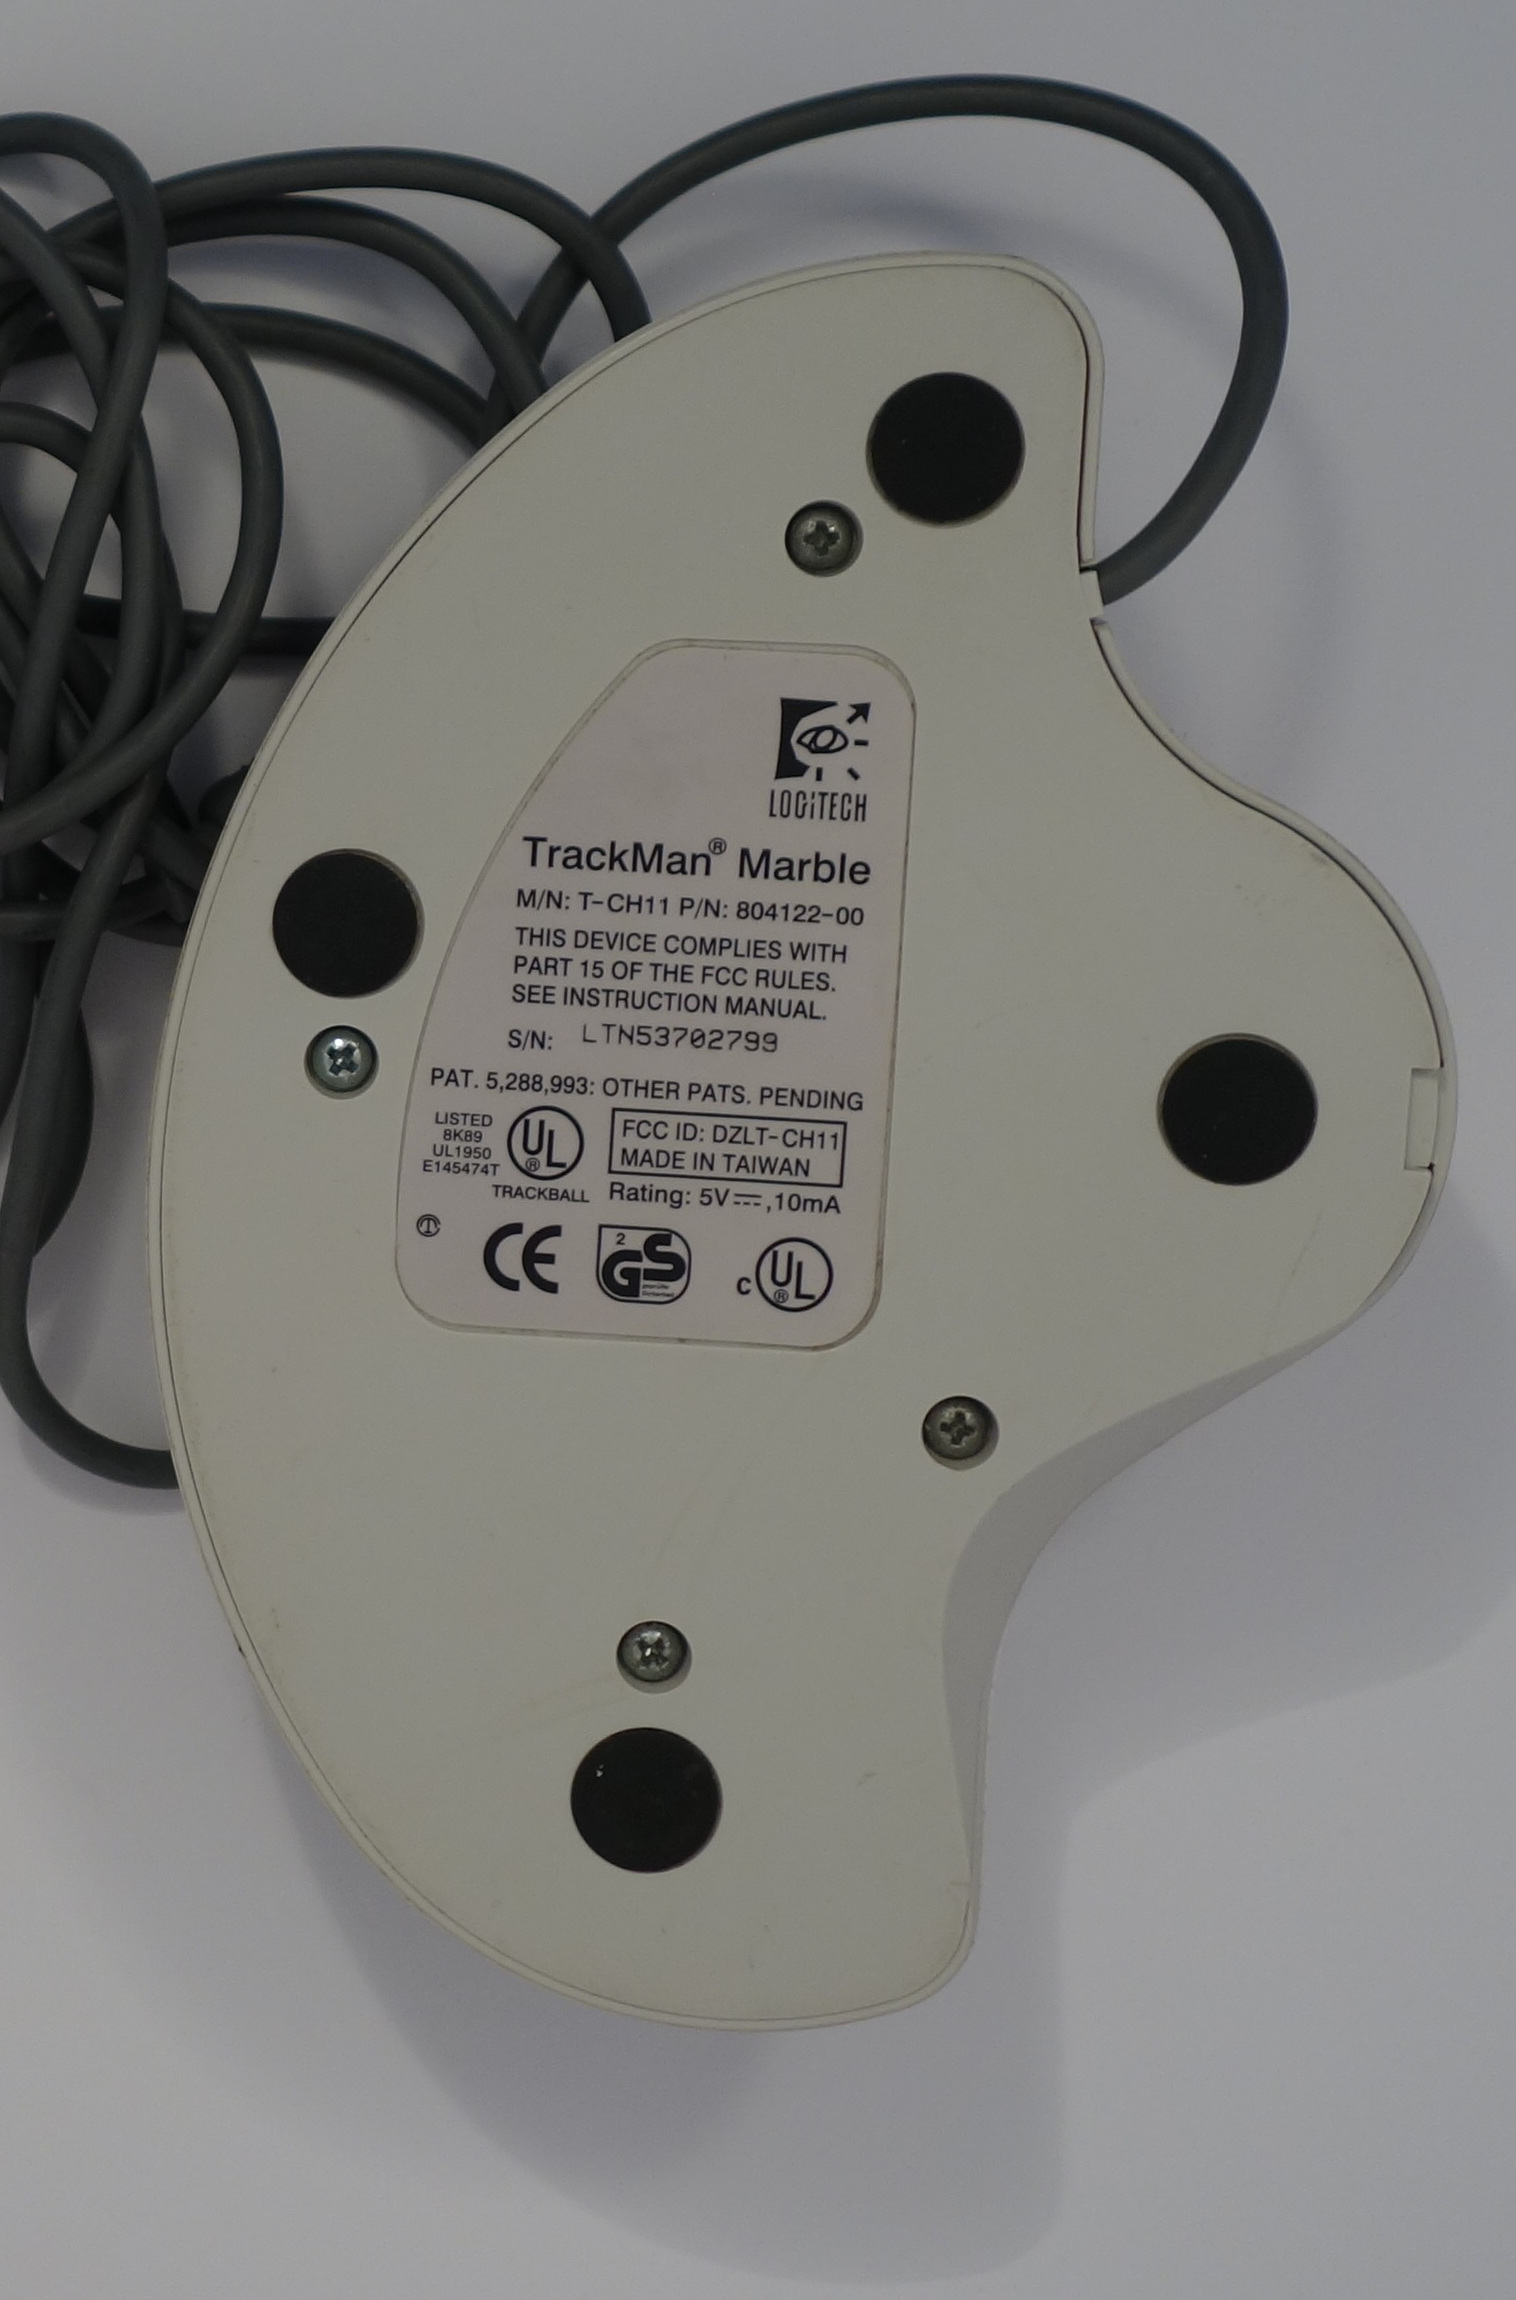
\includegraphics[scale=0.5]{1995_logitech_trackman/2.17.JPG}
%    \caption{Logitech TrackMan bottom view}
%    \label{fig:trackmanBottom}
%\end{figure}

\begin{thebibliography}{9}
\bibitem{marbleAdv} Melissa J. Perenson. New \& improved. News of announced products and upgrades. // PC Magazine, Vol. 14, No. 22. -- December 19, 1995. -- p. 61 -- 66.
\bibitem{logitech25} 25-year category criteria. Logitech’s 25 Most Important Products \url{https://www.logitech.com/lang/pdf/logitech_most_important_products.pdf}
\end{thebibliography}

\end{document}
